\subsection{Огляд можливостей управління транспортними даними}
\label{subsec:route-management-subsection}

Застосунок пропонує комплексний набір функцій управління транспортними даними, які дозволяють адміністраторам підтримувати та оновлювати базу даних транспортних маршрутів, розкладів та іншої пов'язаної з ними інформації. Ці функції дозволяють легко інтегрувати нові маршрути, вносити зміни до існуючих маршрутів та ефективно обробляти зміни в розкладі руху транспорту.

Однією з ключових особливостей функцій управління транспортними даними є можливість додавання нових транспортних маршрутів до системи. Адміністратори можуть вводити необхідні дані, такі як пункт відправлення, пункт призначення, проміжні зупинки та пов'язану з ними інформацію про розклад для кожного маршруту. Це дозволяє додатку надавати користувачам точні та вичерпні варіанти маршрутів під час пошуку.

Функції управління транспортними даними також включають можливість видалення застарілих або зайвих маршрутів із системи. Це гарантує, що додаток підтримує чисту та актуальну базу даних, підвищуючи ефективність процесу пошуку та покращуючи загальний користувацький досвід.

Для спрощення управління транспортними даними додаток надає інтуїтивно зрозумілі інтерфейси та інструменти, які полегшують навігацію та редагування інформації про маршрути. Адміністратори можуть використовувати ці інтерфейси для візуалізації маршрутів, перегляду розкладів і внесення необхідних змін у зручний для користувача спосіб. Система також може включати механізми перевірки даних для забезпечення точності та узгодженості введеної інформації, мінімізації помилок та покращення цілісності даних.

Використовуючи функції управління транспортними даними, адміністратори можуть ефективно підтримувати та оновлювати транспортні дані в додатку, забезпечуючи користувачам доступ до надійної та актуальної інформації про маршрути. Це дозволяє користувачам приймати обґрунтовані рішення, ефективно планувати свої поїздки та впевнено орієнтуватися в транспортній мережі.

Адміністратор може створювати нові маршрути для того щоб вони потім відображались при пошуку маршрутів

\begin{figure}[!h]
	\centering
	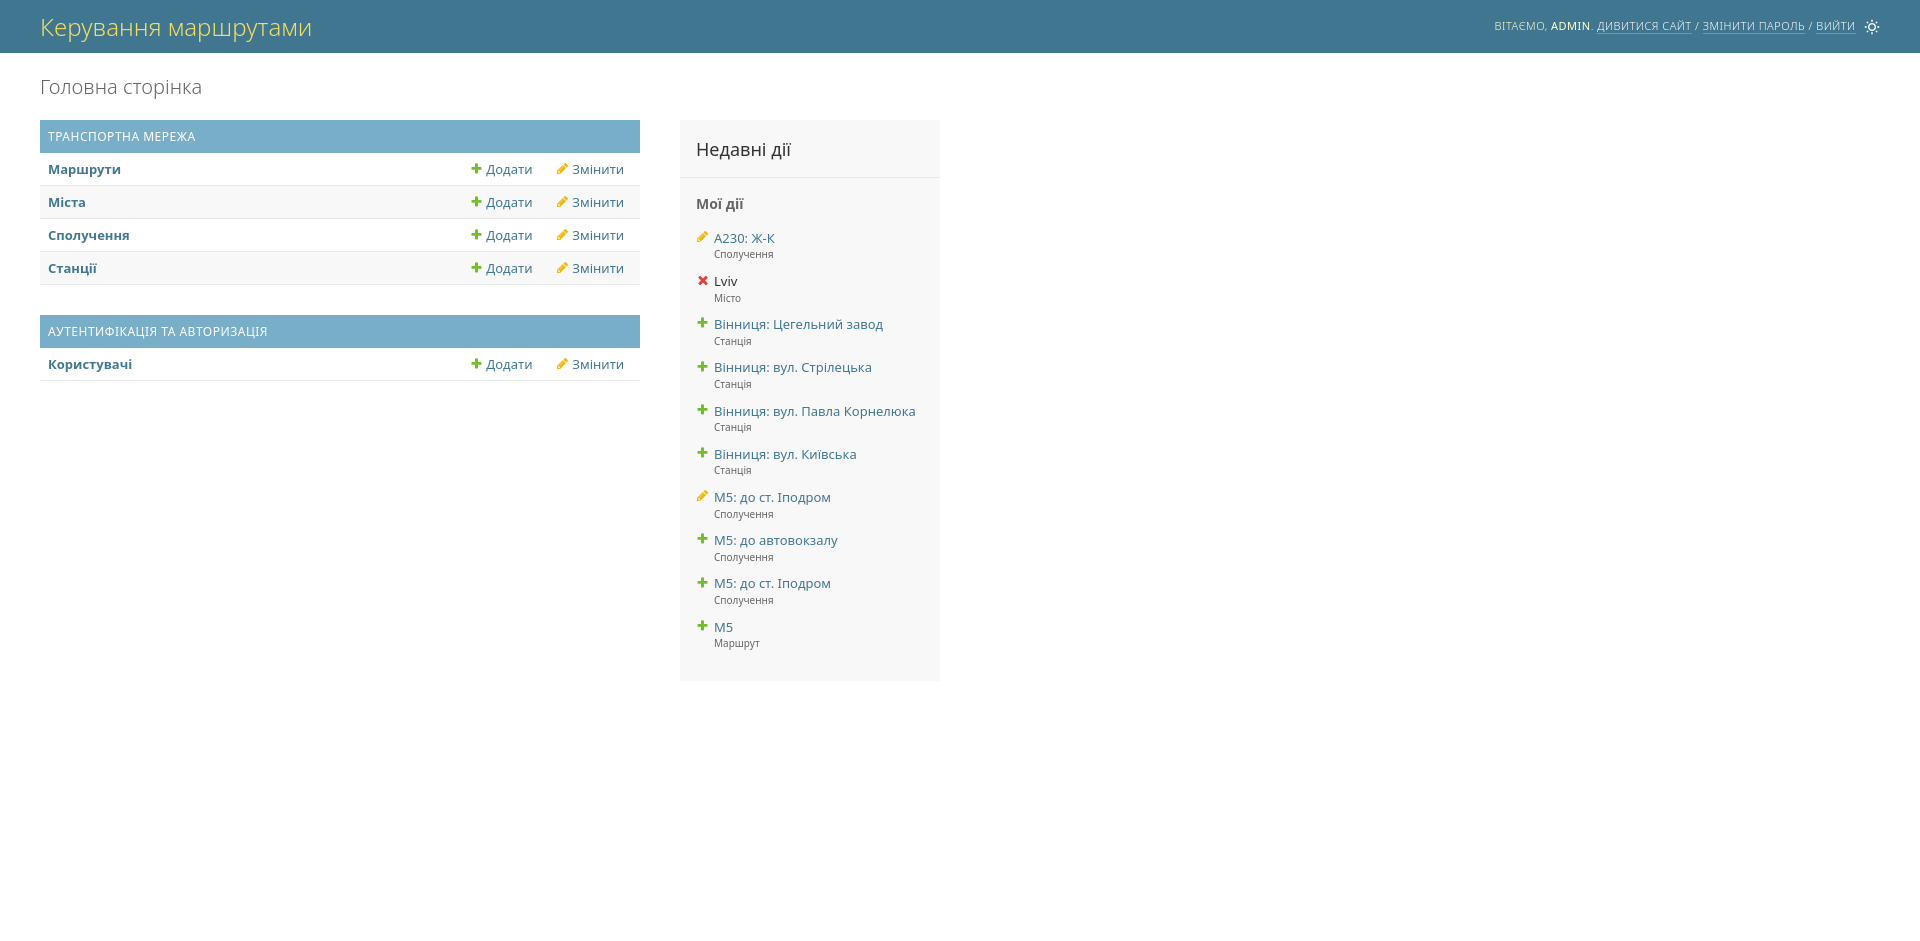
\includegraphics[scale=0.35]{content/chapters/4-results/assets/img/admin_main.png}
	\caption{Головна сторінка інрерфейсу адміна}
	\label{fig:admin_main_page}
\end{figure}

\begin{figure}[!h]
	\centering
	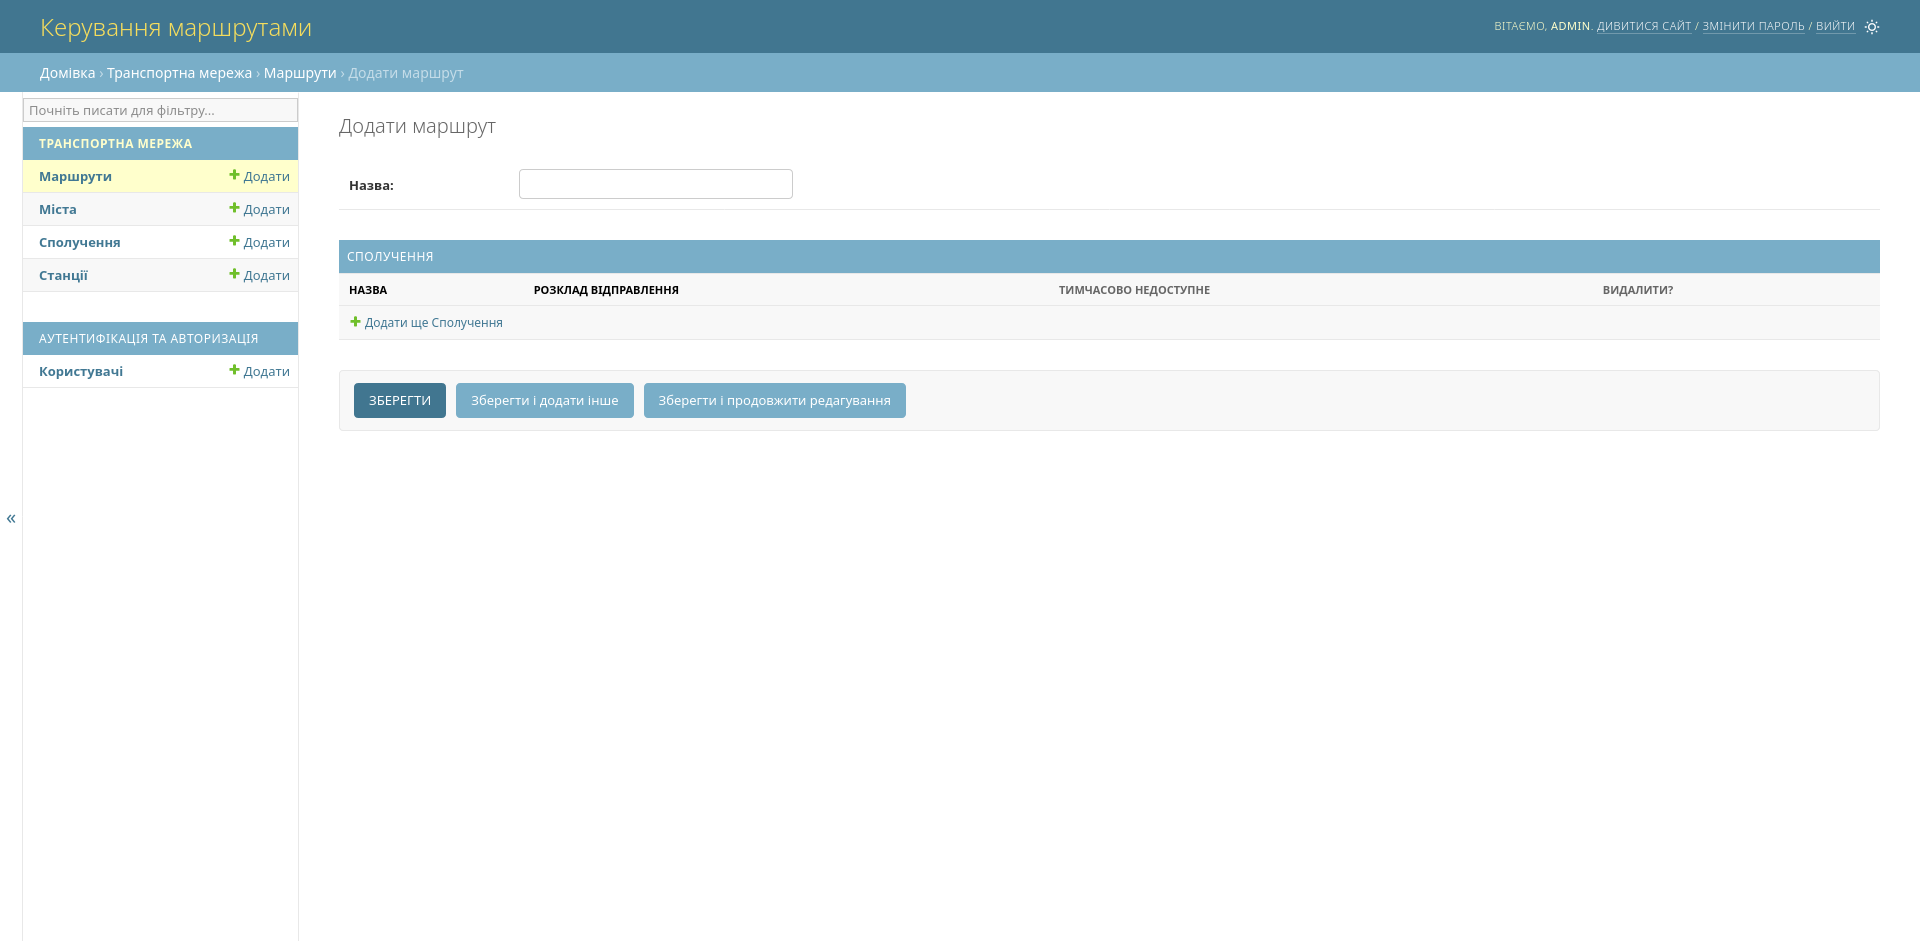
\includegraphics[scale=0.35]{content/chapters/4-results/assets/img/admin_create_r.png}
	\caption{Створення нового маршруту}
	\label{fig:roure_creation_page}
\end{figure}


\begin{figure}[!h]
	\centering
	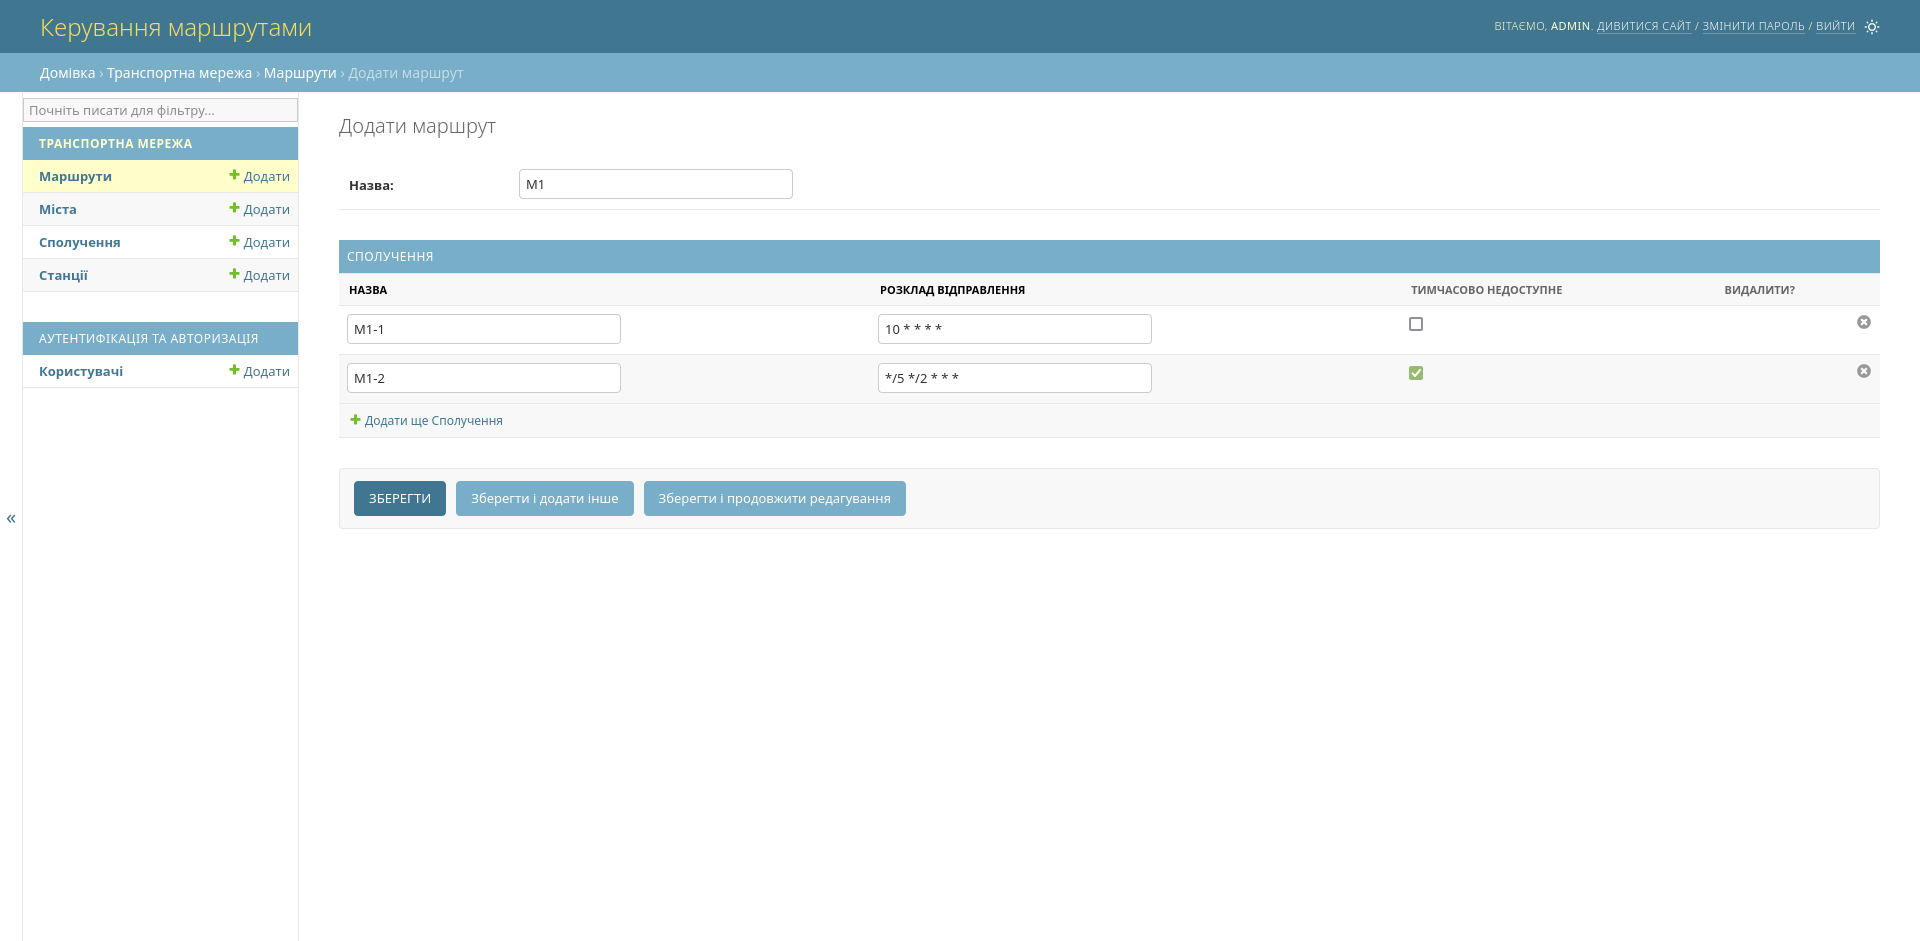
\includegraphics[scale=0.35]{content/chapters/4-results/assets/img/admin_create_R_filled.png}
	\caption{Заповнені поля для створення нового маршруту}
	\label{fig:route_creation_filled_page}
\end{figure}



Після створення маршрутів, їх можна переглядати в списку зі всіма маршрутами.

\begin{figure}[!h]
	\centering
	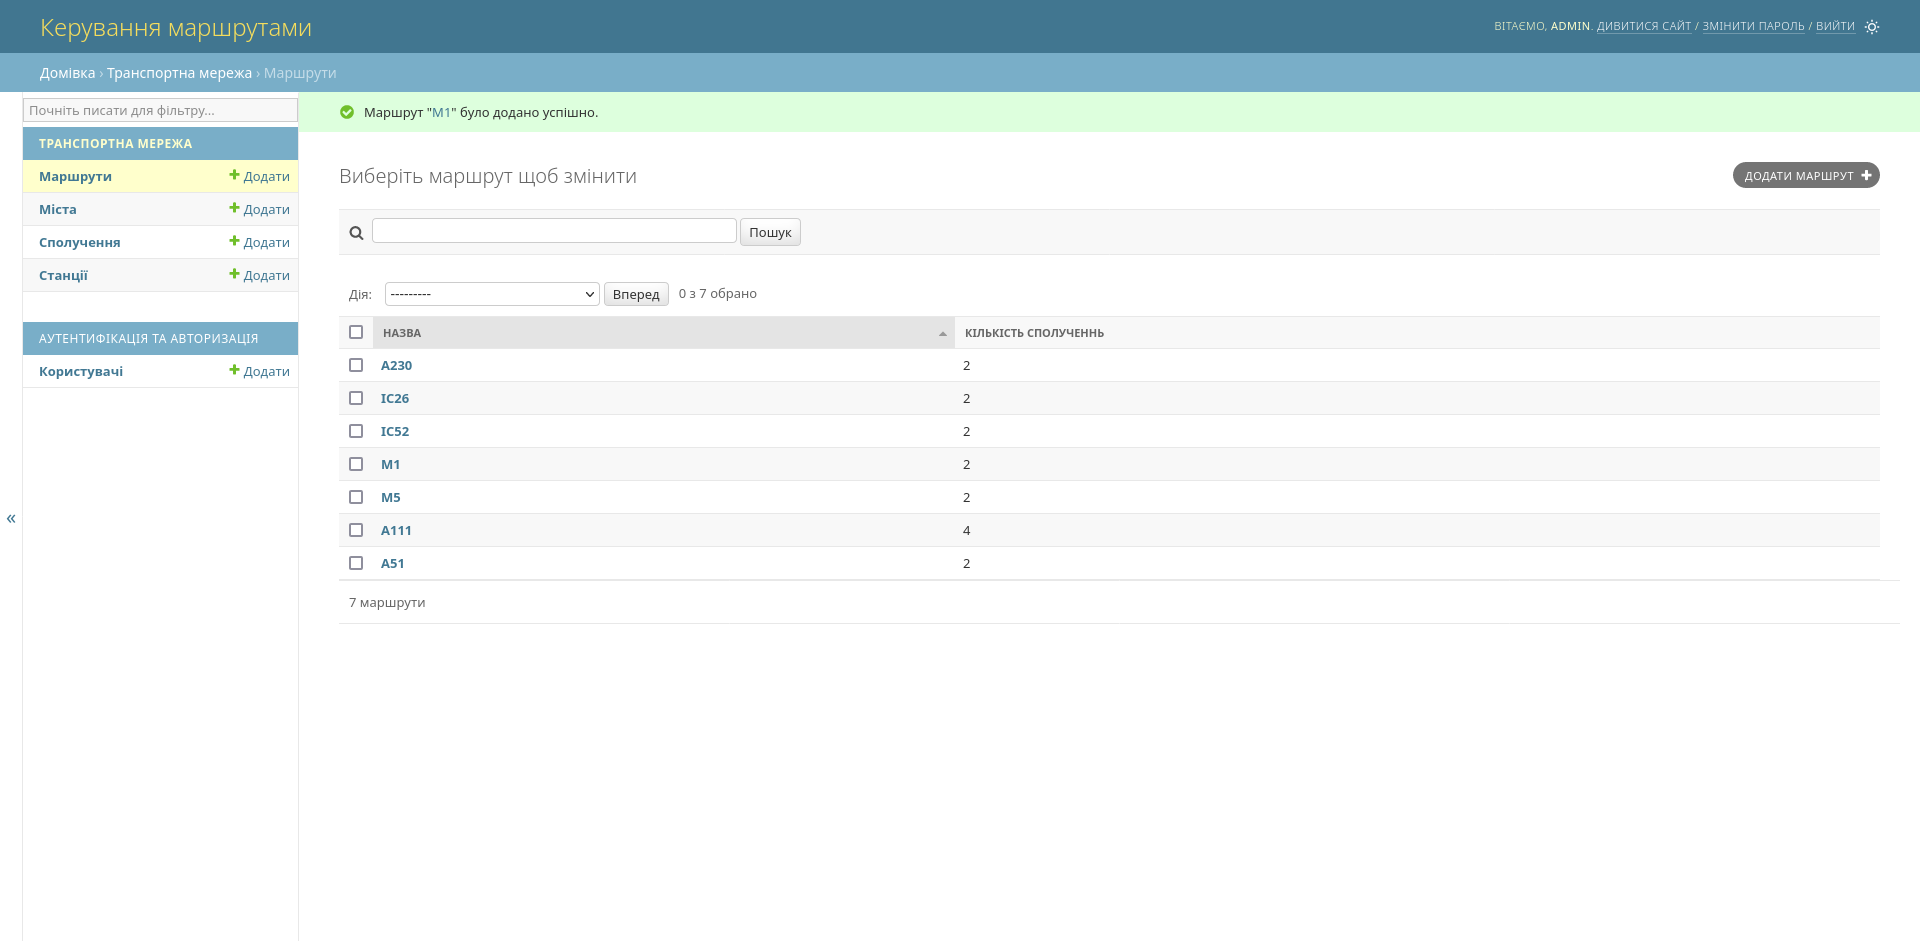
\includegraphics[scale=0.35]{content/chapters/4-results/assets/img/admin_view_r.png}
	\caption{Сторінка зі всіма маршрутами}
	\label{fig:route_display_page}
\end{figure}



Кожен маршрут можна відкрити на окремій сторінці для перегляду деталей  про нього. Якщо в маршруті є помилки, дані про маршрут можна редагувати, чи навіть видалити.

\begin{figure}[!h]
	\centering
	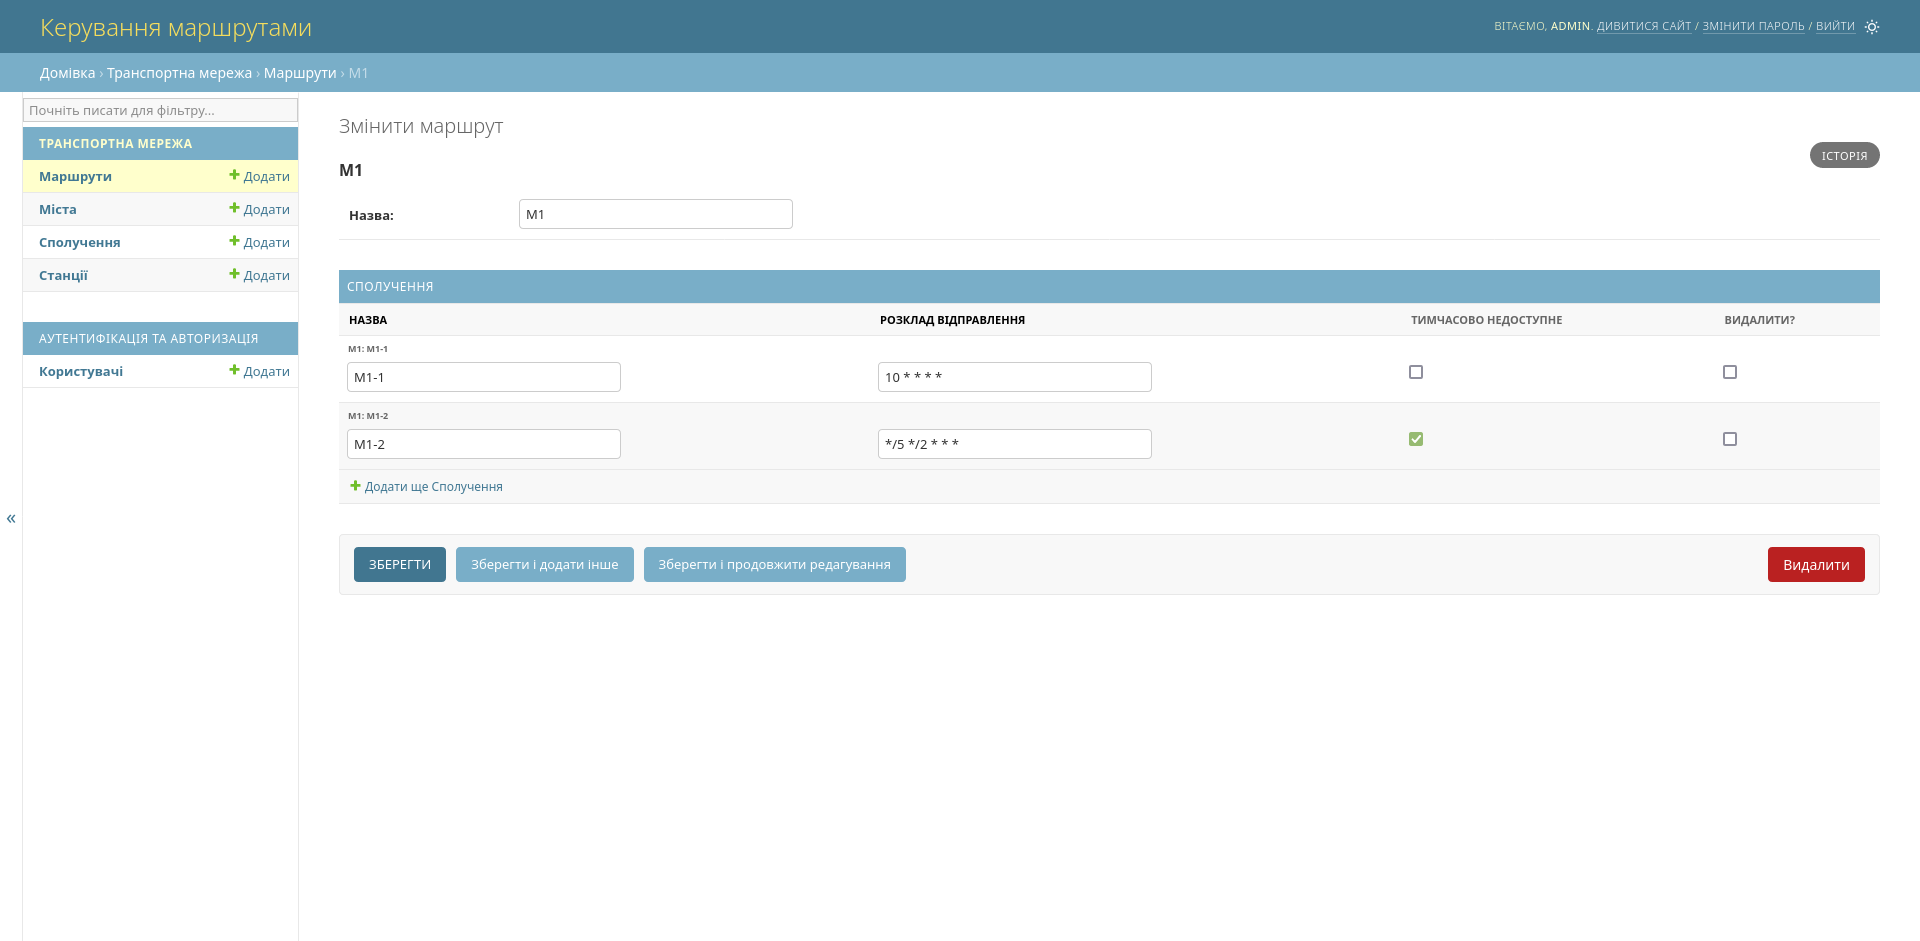
\includegraphics[scale=0.35]{content/chapters/4-results/assets/img/admin_r_details.png}
	\caption{Перегляд деталей про маршрут}
	\label{fig:route_edit_page}
\end{figure}
